\documentclass[a4paper]{article} % Specify A4 paper

% Optional packages
\usepackage[utf8]{inputenc} % Allows UTF-8 input
\usepackage[T1]{fontenc}    % Selects font encodings
\usepackage{amsmath}        % For mathematical formulas
\usepackage{graphicx}       % To include images
\usepackage[ngerman]{babel} % German language support
\usepackage{geometry}       % For page layout adjustments
\usepackage{lipsum}         % For generating dummy text to fill pages
\usepackage{blindtext}      % Another package for dummy text

% Adjust page margins if needed (optional, default article margins are usually fine)
% \geometry{a4paper, margin=2.5cm}

% Document information
\title{Dokumentation zur Pipeline-Architektur}
\author{Ihr Name / Projektgruppe}
\date{\today}

\begin{document}

\section{Praktische Umsetzung: Beispiel einer Datenverarbeitungs-Pipeline}
\subsection{Gesamtarchitektur}
Um die Konzepte der Pipeline-Architektur zu verdeutlichen, ist dieser Ausarbeitung eine Beispielanwendung beigelegt. Diese Beispielanwendung verdeutlicht mithilfe einer Architektur, wie eine Pipeline aufgebaut ist und was deren vorteile sind.
In der Abbildung \ref{fig:application_structure} ist der Aufbau zu betrachten. Im Bereich Pipeline Start befinden sich zwei Knöpfe Open und Update. Mit Open beginnt der Pipeline Prozess, mit Update wird dieser Aktualisiert. Im Bereich Pipeline Config ist es dem Nutzer möglich verschiedene Pipelinesegmente zu Aktivieren und deren Parameter zu konfigurieren um verschiedene Ergebnisse an den Pipelineverarbeitungen zu erzeugen. Die Verarbeiteten Bilder werden im Nachgang im bereich Ergebnis Ausgabe angezeigt so dass der Benutzer eine Live betrachtung der Pipeline Ergebnisse bekommt.

\begin{figure}[htbp]
    \centering
    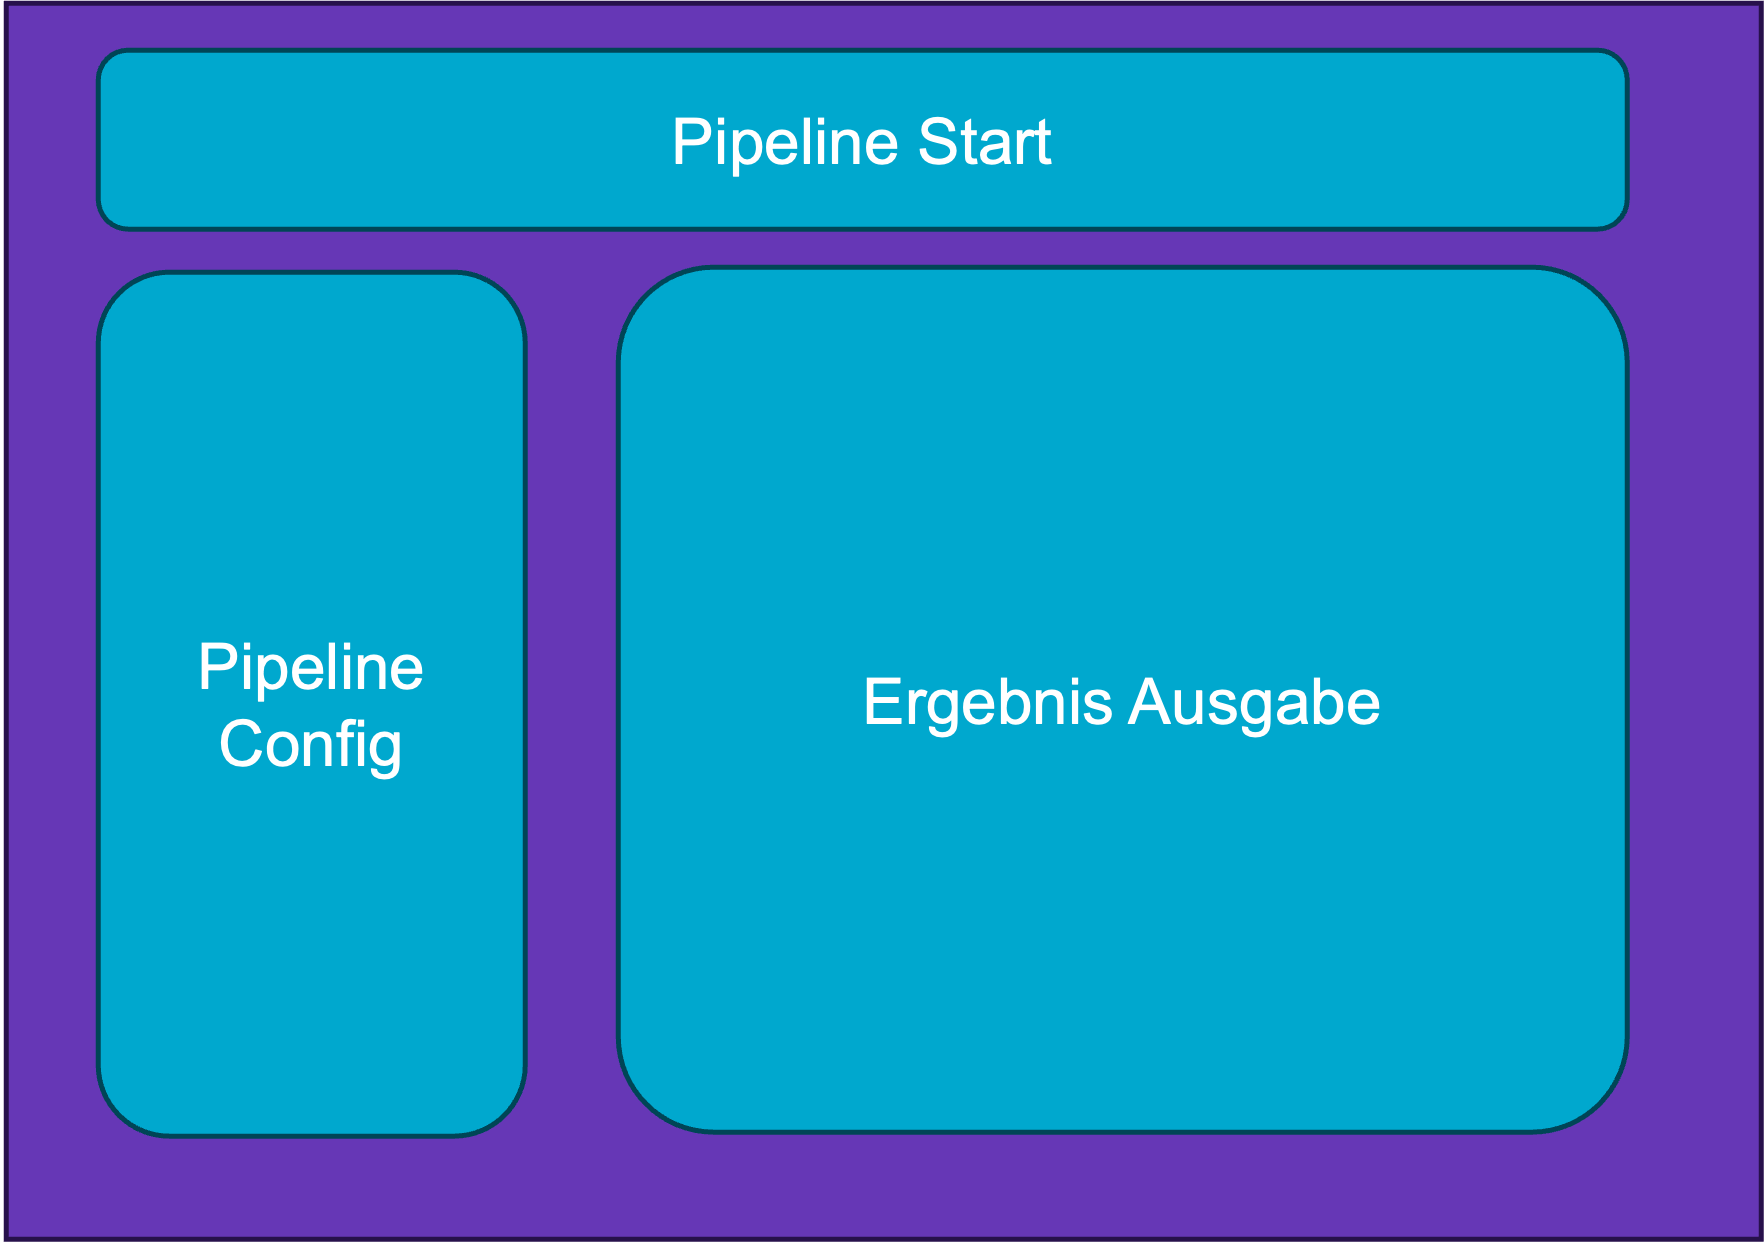
\includegraphics[width=0.8\textwidth]{img/ApplicationStructure.png}
    \caption{Aufbau der Demo GUI.}
    \label{fig:application_structure}
\end{figure}

\begin{samepage}
Die GUI als solches ist nicht Teil der Pipeline. Diese ist nach dem MVC Pattern aufgebaut und nutze lediglich die Pipeline Architektur. Dadurch ist die Pipeline unabhängig von der GUI und kann an anderer stelle wiederverwendet werden. Die Abbildung \ref{fig:gui_pipeline_interface} verdeutlicht diese Trennung, da die GUI lediglich die Pipeline ansteuert und die Ergebnisse anzeigt, ohne direkt in die Logik der Pipeline eingreifen zu können.

\begin{figure}[htbp]
    \centering
    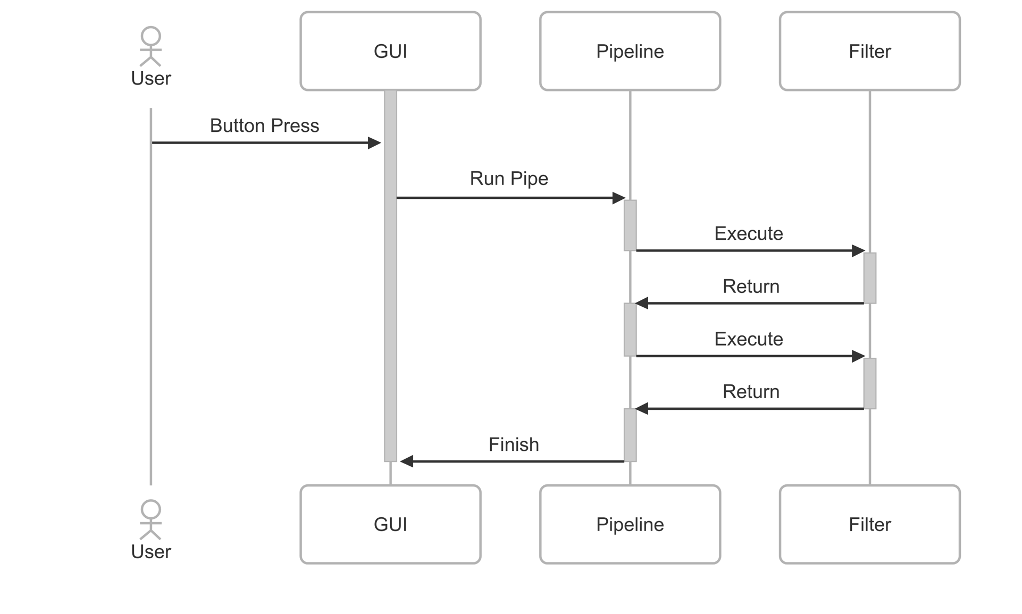
\includegraphics[width=0.8\textwidth]{img/GuiPipelineInterface.png}
    \caption{Kommunikation zwischen GUI und Pipeline.}
    \label{fig:gui_pipeline_interface}
\end{figure}
\end{samepage}

Wird durch den Open Button die Pipeline gestartet öffnet sich zuerst ein Dateiauswahldialog in welchem der Benutzer die zu verarbeitende Datei auswählen kann. Dies ist der Einstieg in die Pipeline welche aus den folgenden Stufen besteht:

\begin{enumerate}
    \item \textbf{Loader:} In dieser ersten Stufe werden die Rohdaten von der Datenquelle (z.B von Bilddateien wie JPG, SVG, etc.) eingelesen. Dies beinhaltet das Öffnen der Datei und das Parsen des Inhalts in eine interne Datenstruktur.
    \item \textbf{Transformer:} Auf die Daten werden nun Filter angewendet. Das kann simple Bildbearbeitungsprozesse wie das Drehen oder Flippen des Bildes sein. Es können aber auch komplexere Transformationen wie eine Bildanalyse via eines neuronalen Netzes sein, um bestimmte Merkmale zu extrahieren oder zu klassifizieren.
    \item \textbf{Tester:} Testeranwendungen überprüfen ob die Transformer korrekt angewendet wurden und die Ergebnisse zu Erwartungswerten passen.
    \item \textbf{Consumer:} Die verarbeiteten Ergebnisse werden persistiert (z.B. in einer Datenbank oder Datei gespeichert) oder an nachfolgende Systeme zur weiteren Verwendung übergeben. Das kann zum Beispiel eine GUI sein.
\end{enumerate}


\subsection{Implementierung der Pipeline-Steuerung: Die Wrapper-Klasse}
Die Implementierung einer Pipeline kann dabei auf unterschiedliche Weisen erfolgen. Welche unterschiedliche Vor- und Nachteile in bezug auf Flexibilität, Erweiterbarkeit und Coding aufwand haben. Geläufige Ansätze sind:

\begin{itemize}
    \item \textbf{Direkte Implementierung im Code:} Die Abfolge der Stufen wird direkt im ausführenden Code definiert. Dies ist einfach für kleine Pipelines, kann aber bei wachsender Komplexität unübersichtlich und schwer wartbar werden.
    \item \textbf{Konfigurationsbasierter Ansatz:} Die Pipeline-Struktur wird in einer externen Datei (z.B. YAML, JSON) definiert und zur Laufzeit geladen. Dies bietet hohe Flexibilität und ermöglicht Anpassungen ohne Code-Änderungen, erfordert jedoch zusätzlichen Aufwand für das Parsen und Validieren der Konfiguration.
    \item \textbf{Wrapper-Klasse:} Eine dedizierte Klasse kapselt die Logik zur Verwaltung der Stufen (Hinzufügen, Reihenfolge) und zur Ausführung der Pipeline. Dies fördert die Struktur, Kapselung und Wiederverwendbarkeit.
\end{itemize}

Für die Beispielanwendung ist eine Wrapper-Klasse der beste Ansatz. Durch die Wrapper-Klasse ist die Pipeline von der GUI getrennt und trotzdem einfach zugreifbar, ermöglicht es aber gleichzeitig, dynamische Änderungen vorzunehmen. Die Kernidee dabei ist es, eine Klasse (z.B. `Pipeline`) zu erzeugen. Diese Klasse verwaltet eine Liste von Pipeline-Stufen, welche im Folgenden als `Stage` bezeichnet werden. Jede `Stage`, die implementiert wird, leitet von der abstrakten Basisklasse `Stage` ab. Dadurch muss jede konkrete Stufe die definierte Methode `process` implementieren, was sicherstellt, dass alle Stufen einheitlich behandelt und von der `Pipeline`-Klasse aufgerufen werden können.

Die Wrapper-Klasse enthält zudem Mechanismen, um sicherzustellen, dass nur valide Stufen hinzugefügt werden. Dies wird durch Typ-Prüfungen realisiert, wie im folgenden Python-Codeausschnitt für die add\_stage-Methode gezeigt:

\begin{figure}[htbp]
    \centering
    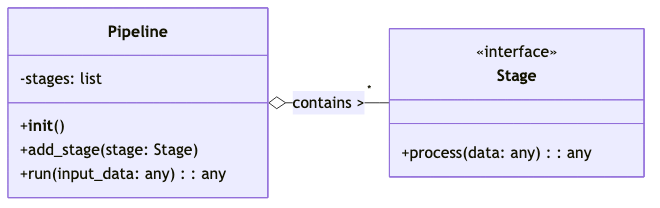
\includegraphics[width=0.8\textwidth]{img/wrapper.png}
    \caption{Klassendiagramm der Pipeline Wrapper-Klasse (`Pipeline`) und der abstrakten Stufenklasse (`Stage`).}
    \label{fig:wrapper}
\end{figure}

Damit änderungen in einer Stage nur gezielt nachfolgende Stages beeinflussen ist es Sinnvoll eine Datenklasse zu definieren um den Transfer zwischen den Stages zu steuern. In der Beispielanwendung übernimmt dies die PipeDataClass. Jede Stage erwartet eine Instanz dieser Klasse als Parameter in der `process`-Methode und gibt eine modifizierte Instanz zurück. Dadurch wird sichergestellt, dass die Daten zwischen den Stufen konsistent und nachvollziehbar bleiben.

Da die Demo eine Bildbearbeitung demonstriert muss zusätzlich zwischen Globalen Änderungen und Lokalen Änderungen unterschieden werden. Globale Änderungen sind dinge welche das gesamte Bild beeinflussen. Dies kann beispielsweise das Drehen des Bildes sein. Lokale Änderungen sind dagegen Dinge welche das Bild bearbeiten, von denen aber nicht gewünscht ist, dass diese Nachfolgende Filter beeinflussen. Darunter fallen Filter wie Bounding Boxes von Neuronalen Netzen oder Poster welche per Arucomarker im Bild platziert werden. 
Diese könnten Nachfolgende Filter beeinflussen obwohl diese im gegensatz zu Rotationen keinen Vorteil für die Nachfolgenden Stages haben. Daher greifen Globale Änderungen auf das base_image_from_source direkt zu, während Lokale Änderungen ihre Änderungen per 

add\_optional\_layer in eine Liste von optionalen Layern hinzufügen. Diese optionalen Layer werden dann in der Consumer Stage zusammengeführt und als Ergebnis ausgegeben.

\ref{fig:application_structure}

\begin{verbatim}
def add_stage(self, stage:Stage):
    if(not issubclass(stage, Stage)):
        raise TypeError("stage must be an instance of Stage")
\end{verbatim}\

Diese Sicherung wird in Python durch das Prüfen des Klassentyps (issubclass) sichergestellt. Wird eine Klasse übergeben welche keine Subklasse von Stage ist wird ein TypeError geworfen. Dies geschieht bei issubclass selbst bei einer erzeugten Instanz von Stage selbst.

\subsection{Factory Pattern zur dynamischen Komponentenauswahl}
Ein weiteres nützliches Entwurfsmuster, das häufig in Verbindung mit der Pipeline-Architektur eingesetzt wird, ist das Factory Pattern. Dieses Muster gehört zu den Erzeugungsmustern und dient dazu, Objekte zu erstellen, ohne die genaue Klasse des zu erstellenden Objekts im Voraus festlegen zu müssen. Stattdessen wird die Verantwortung für die Objekterzeugung an eine spezialisierte "Factory"-Klasse oder -Methode delegiert.

Das Factory Pattern ermöglicht eine signifikante Entkoppelung des aufrufenden Codes (in unserem Fall die Pipeline oder eine ihrer Stufen) von der konkreten Implementierung der zu erzeugenden Objekte. Die Factory fungiert als zentraler Punkt für die Erzeugung von Objekten eines bestimmten Typs oder einer bestimmten Schnittstelle. Abhängig von den übergebenen Parametern oder dem Kontext entscheidet die Factory, welche spezifische Unterklasse instanziiert und zurückgegeben werden soll.

\subsubsection{Anwendung im Datenlader}
In unserem Beispiel einer Datenverarbeitungs-Pipeline findet das Factory Pattern eine praktische Anwendung, insbesondere bei der Funktion zum Auslesen der Sensordateien. Unterschiedliche Sensoren oder Datenquellen können ihre Daten in verschiedenen Formaten bereitstellen (z.B. CSV, JSON, XML, Binärformate). Anstatt die Logik zur Erkennung und Verarbeitung jedes Formats direkt in die Pipeline-Stufe einzubetten, die die Daten lädt, wird eine `LoaderFactory` eingesetzt.

Der Ablauf ist typischerweise wie folgt:
\begin{enumerate}
    \item Eine vorherige Pipeline-Stufe oder der Initialaufruf übergibt den Dateipfad oder eine andere Kennung der zu ladenden Daten an die Stufe, die für das Laden zuständig ist.
    \item Diese Ladestufe delegiert die Erzeugung des passenden Ladeobjekts an die `LoaderFactory`. Sie übergibt dabei relevante Informationen, wie z.B. den Dateipfad oder explizit das Dateiformat.
    \item Die `LoaderFactory` analysiert die übergebenen Informationen (z.B. die Dateiendung wie `.csv` oder `.json`).
    \item Basierend auf dieser Analyse instanziiert die Factory ein konkretes Ladeobjekt (z.B. eine Instanz von `CsvLoader` oder `JsonLoader`), das eine gemeinsame Schnittstelle (z.B. `DataLoader`) implementiert.
    \item Die Factory gibt das erzeugte Ladeobjekt an die aufrufende Pipeline-Stufe zurück.
    \item Die Pipeline-Stufe verwendet nun das erhaltene Ladeobjekt, um die Daten zu laden, ohne die spezifische Implementierung des Laders kennen zu müssen. Sie interagiert nur über die definierte Schnittstelle (`DataLoader`).
\end{enumerate}

Abbildung \ref{fig:loaderFactory} illustriert diesen Entscheidungsprozess innerhalb der Factory. Die Factory prüft das angeforderte Format und wählt den entsprechenden Loader aus. Sollte kein passender Loader für das angeforderte Format registriert sein oder die Datei nicht existieren, wird typischerweise ein Fehler ausgelöst oder ein Null-Objekt zurückgegeben, um das Problem zu signalisieren.

\begin{figure}[htbp] % h: here, t: top, b: bottom, p: page of floats
    \centering % Center the image
    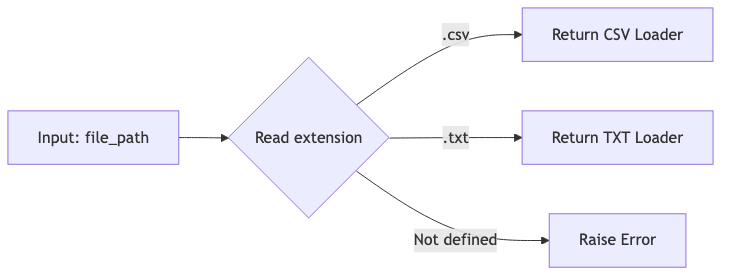
\includegraphics[width=0.8\textwidth]{img/LoaderFactory.png} % Include the image, adjust width as needed
    \caption{Entscheidungsdiagramm der LoaderFactory zur Auswahl des passenden Datenladers basierend auf dem Dateiformat.} % Add a caption
    \label{fig:loaderFactory} % Add a label for referencing
\end{figure}

\subsubsection{Vorteile des Factory Patterns in der Pipeline}
Der Einsatz des Factory Patterns in diesem Kontext bietet mehrere signifikante Vorteile:

\begin{itemize}
    \item \textbf{Entkoppelung:} Der Code der Pipeline-Stufe, die Daten lädt, ist von den konkreten Ladeimplementierungen entkoppelt. Er interagiert nur mit der Factory und der abstrakten `DataLoader`-Schnittstelle.
    \item \textbf{Flexibilität und Erweiterbarkeit (Open/Closed Principle):} Das Hinzufügen der Unterstützung für neue Dateiformate wird erheblich vereinfacht. Es muss lediglich eine neue `DataLoader`-Unterklasse (z.B. `XmlLoader`) implementiert und die `LoaderFactory` entsprechend erweitert werden, um diese neue Klasse bei Bedarf zu instanziieren. Der Code der Pipeline-Stufe selbst muss nicht modifiziert werden. Das System ist offen für Erweiterungen, aber geschlossen für Modifikationen.
    \item \textbf{Zentralisierung der Erzeugungslogik:} Die Logik zur Entscheidung, welcher Loader wann erstellt wird, ist an einem einzigen Ort – der Factory – konzentriert. Dies verbessert die Wartbarkeit und Übersichtlichkeit des Codes. Änderungen an der Erzeugungslogik müssen nur an dieser zentralen Stelle vorgenommen werden.
    \item \textbf{Verbesserte Testbarkeit:} Die einzelnen Loader-Klassen sowie die Factory selbst können isoliert getestet werden.
    \item \textbf{Wiederverwendbarkeit:} Die Factory und die Loader-Klassen können potenziell auch in anderen Teilen der Anwendung oder in anderen Projekten wiederverwendet werden. Wie bereits erwähnt, ist dies besonders nützlich, wenn die Ladefunktionalität als Teil eines wiederverwendbaren Moduls, Plugins oder Pakets (Pip Package) bereitgestellt wird. Entwickler, die das Paket nutzen, können eigene Loader hinzufügen und über die Factory registrieren (falls die Factory dies unterstützt), ohne den Kerncode des Pakets ändern zu müssen.
\end{itemize}

Zusammenfassend lässt sich sagen, dass das Factory Pattern die Struktur der Pipeline verbessert, indem es die Erzeugung von Komponenten wie Datenladern flexibler, wartbarer und erweiterbarer gestaltet. Es fördert ein sauberes Design, indem es Abhängigkeiten reduziert und Verantwortlichkeiten klar trennt.


\end{document}